\documentclass{article} % For LaTeX2e
\usepackage{nips13submit_e,times}
\usepackage{hyperref}
\usepackage{url}
\usepackage{graphicx}
\usepackage{epstopdf}
\usepackage{listings}
\lstset{language=Matlab}
\lstset{breaklines}
\lstset{extendedchars=false}
\usepackage{amsmath}
\usepackage{txfonts}
\usepackage{subfigure}
\usepackage{mathrsfs}



\title{Convolutional Neural Network and Convex optimization}


\author{
Si Chen  and   Yufei Wang\\
Department of Electrical and Computer Engineering\\
University of California San Diego\\
\texttt{\{sic046, yuw176\}@ucsd.edu}          \\
}

% The \author macro works with any number of authors. There are two commands
% used to separate the names and addresses of multiple authors: \And and \AND.
%
% Using \And between authors leaves it to \LaTeX{} to determine where to break
% the lines. Using \AND forces a linebreak at that point. So, if \LaTeX{}
% puts 3 of 4 authors names on the first line, and the last on the second
% line, try using \AND instead of \And before the third author name.

\newcommand{\fix}{\marginpar{FIX}}
\newcommand{\new}{\marginpar{NEW}}

\nipsfinalcopy % Uncomment for camera-ready version

\begin{document}


\maketitle
\begin{abstract}
%We model the relationship between sentences and their punctuation labels using conditional random fields. Some feature functions are hand-designed and others are generated by templates. We train the same model by stochastic gradient ascent, Collins Perceptron and contrastive divergence respectively and compare their performance. On the provided dataset, we achieve word-level accuracy of 94.56\%. At last, we propose a heuristic that can deal with cost-sensitive tasks.   
Latent Dirichlet allocation(LDA) is a generative topic model to find latent topics in a text corpus. It can be trained via collapsed Gibbs sampling. In this project, we train LDA models on two datasets, Classic400 and BBCSport dataset. We discuss possible ways to evaluate goodness-of-fit and to detect overfitting problem of LDA model, and we use these criteria to choose proper hyperparameters, observe convergence, and evaluate the models, the criteria we use include perplexity, VI-distance, visualization of clustering results, and highest-probability words. 

\end{abstract}
\section{Introduction}

Deep learning


Convex optimization


SVM-loss



%Latent Dirichlet allocation introduced by \cite{blei} is a generative probabilistic model for collection of discrete data, such as text corpora.It assumes each word is a mixture over an underlying set of topics, and each topic is a mixture over a set of topic probabilities. Evaluating the models is a tough issue. There are several types of methods that people use: The models can be applied to some tasks such as document classification, where the performance can be easily evaluated; Several methods estimate the likelihood of held-out documents; Subjective judgement can be made by examine word and document similarities. In this project, we learn the models of two datasets, Classic400 and BBCSport dataset, by collapsed Gibbs sampling, and use several methods to evaluate the models, including perplexity, VI-distance, visualizing result and highest-probability words.
\par
%This report is organized as follows. Section 2 gives a brief overview of LDA model and training process, and introduces several methods to evaluate goodness-of-fit and check overfitting. We describe some implementation details in Section 3. In Section 4, we describe the design of our experiments. Section 5 shows the experiment results with discussions. Finally, we draw some conclusions in Section 6.

\section{Sub-model Convolutional Network}
\subsection{Theoretical basis: Convolutional neural network}
Convolutional neural networks(CNN) are a special kind of deep neural networks. It exploits local correlation by enforcing a local connectivity pattern between neurons of adjacent layers. For a certain hidden layer $m$, the hidden units in it are connected to a local subset of units in the $(m-1)$th layer. Additionally, each sparse filter $h_{i}$ is replicated across the entire visual field. The replicated units share the same parametrization, i.e. the same weight vector and same bias. The layer is called feature map. 
\par
Mathematically, a feature map $h^{k}$ is obtained by convolving the input with a linear filter, adding a bias term and then applying a non-linear function, it can be shown as follow:
\begin{equation}
h^{k}_{ij}=\textup{f}((W^{k}*x)_{ij}+b_{k})
\end{equation}
where $W^{k}$ and $b_{k}$ are weight and bias of $k$th feature map, and $\textup{f}(\cdot)$ is the nolinearity. In our experiments, Rectified Linear Units(ReLU) nonlinearity is used, which has been shown to be more efficient than conventional function $\textup{tanh}(\cdot)$.\cite{imagenet} ReLU nonlinearity is as follow:
\begin{equation}
f(x)=\textup{max}(0,x)
\end{equation}
\par
Another important type of layers is pooling. It is a form of non-linear down-sampling. There are several types of pooling, two common types of which are max-pooling and average-pooling. They partition the input image into a set of non-overlapping or overlapping rectangles and outputs the maximum/average value for each such sub-region. By pooling, the model can reduce the computational complexity for upper layers, and can provide a form of translation invariance. 
\par
Typically, the last layer of a CNN is a logistic regression layer. Each unit of the output reflects a class membership probability:
\begin{equation}
P(Y=i|x,W,b)=softmax_{i}(Wx+b)=\frac{e^{W_{i}x+b_{i}}}{\sum _{j}e^{W_{j}x+b_{j}}} 
\end{equation}
\par
The parameters of the network are trained using back propagation\cite{backprop}. The loss function used for training is the negative-log likelihood of the training dataset $D$ under the model:
\begin{equation}
L = \sum_{i=0}^{|D|}\textup{log}(P(Y=y^{(i)}|x^{(i)},W,b))
\end{equation}
\par
Finally, the prediction of the model is done by taking the argmax of the vector of $P(Y=i|x,W,b)$:
\begin{equation}
y_{pred}=\textup{argmax}_{i}P(Y=i|x,W,b)
\end{equation}

\subsection{Overall architecture}
The overall architecture of our CNN is shown in Figure~\ref{fig1}. There are three convolutional layers and pooling layers alternatively. Overlapping pooling is performed. Each pooling layer consists of a grid of pooling units spaced $s=2$ pixels apart, each summarizing a neighborhood of size $3\times3$ centered at the location of the pooling unit.

\begin{figure}
\centering
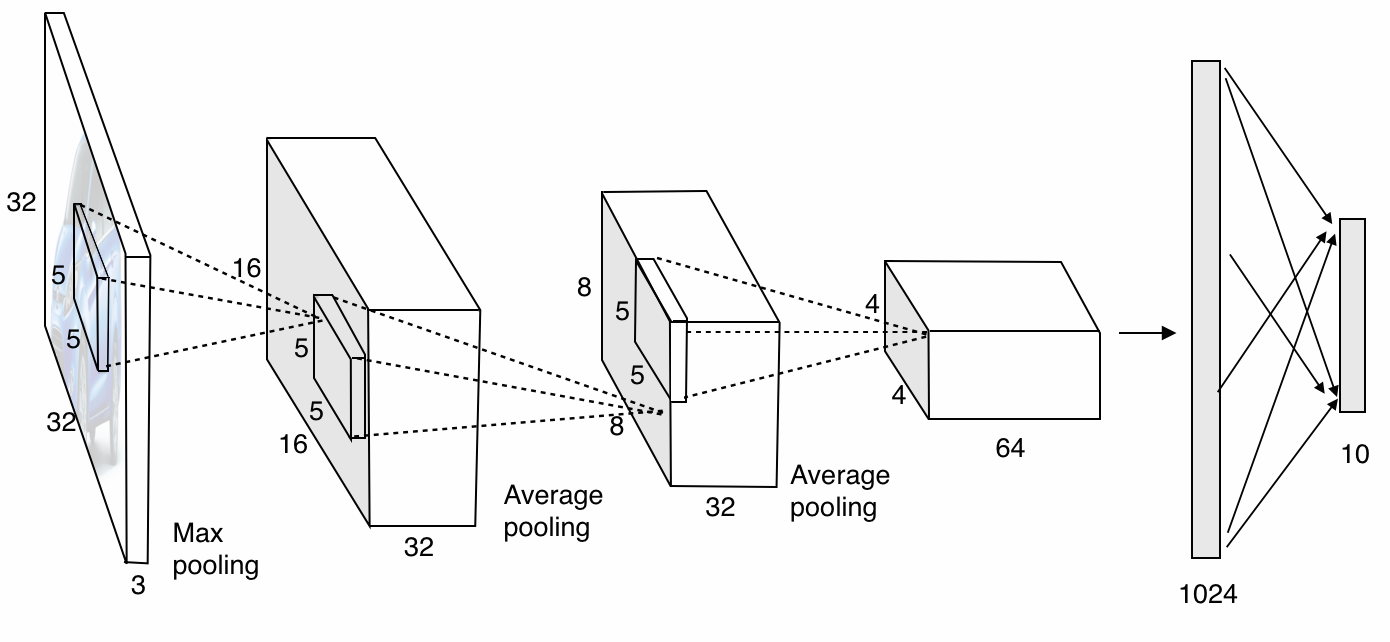
\includegraphics[width=1\textwidth]{architecture}
\caption{The architecture of our CNN.}
\label{fig1}
\end{figure}
\subsection{Sub-model combination}
Let's focus on the penultimate layer in our CNN architecture (Figure~\ref{fig1}). We refer to the already trained CNN model in Figure~\ref{fig1} as the original model. There are totally 1024 units in the penultimate layer, each of which votes for the class membership probabilities $P(Y=i|x,W,b)$, and the importance of each unit's vote is weighted by $W_{ij}$.  The 1024-unit vector of the penultimate layer is denoted as $h_{orig}$.
\par
Now we define a sub-model $m_{i}$ as randomly setting units as zero in the penultimate layer with chance of 50\%, and the remaining units are multiplied by 2:
\begin{equation}
P(h_{m_{i}}^{j}=2h_{orig}^{j})=P(h_{m_{i}}^{j}=0)=\frac{1}{2}.
\end{equation}
where  $h_{m_{i}}$ is the 1024-unit vector of the sub-model $m_{i}$, and $h_{(\cdot)}^{j}$ is the $j$th element of the vector. 
\par
Therefore, the original model can be viewed as a combination of all the possible sub-models:
\begin{equation}
h_{orig} = \lim_{n \to \infty }\frac{1}{n}\sum_{i=1}^{n}h_{m_{i}}=E\left [ h_{m_{i}} \right ]
\end{equation}
For each sub-model, the class membership probability output is denoted as $P_{m_{i}}$. Rather than combining the penultimate layers $h_{m_{i}}$ of the sub-models, we explore the weighted combination of output layer $P_{m_{i}}$ of sub-models:
\begin{equation}
P_{comb} = \sum_{i=1}^{n}l_{i}P_{m_{i}}
\end{equation}
where $l_{i}$ is the weight of each model $m_{i}$, and $P_{comb}$ is the class membership probabilities of the weighted combined model.
\par
Given a set of sub-models $m_{i}, (i = 1,2, ... ,n)$ extracted from the original model $m_{orig}$, the optimal weight $l_{i}$  can be obtained by the following optimization problem:
\par
\setlength{\parindent}{3em}
minimize $\sum_{i=1}^{N}\left \| l^{t}\cdot P_{i}-y_{i} \right \|_{2}^{2}$
\setlength{\parindent}{3em}
subject to $l\succeq 0$

\subsection{Dropout and sub-models}


\section{Convex Loss functions}
Deep neural network is well-known for its highly non-convexity. But we can still borrow some ideas from the convex optimization literature, where people have found many useful convex loss functions for classification tasks. In this section, we will talk about three different convex loss functions, and discuss how to use them in multiclass classification problem within the deep learning architecture.


\subsection{Cross Entropy}
Cross entropy (CE) is the most standard loss function for neural networks, which is defined by:
\begin{equation}
H(p,q) = - \sum_{x}p(x)log q(x),
\end{equation}
where $p$ and $q$ are ground-truth posterior probability and estimated posterior probability respectively. CE can be directly used for multiclass classfication. This has been discussed in Section 2.1. 

\subsection{Hinge Loss}
Hinge loss is widely used in Support Vector Machines (SVMs). Given training data and its corresponding labels ($x_{n}$, $y_{n}$), $n=1,...,N$, $x_{n} \in R^{D}$, $t_{n} \in {-1,+1}$, for a binary classification problem, SVMs learning includes the following convex optimization:
\begin{equation}
\begin{array}{rrclcl}
\displaystyle \min_{w,\psi} & \multicolumn{3}{l}{ \frac{1}{2} w^{T}w +   C\sum_{n=1}^{N}\psi_{n}}\\
\textrm{s.t.} & w^{T}x_{n}t_{n}& \geq & 1-\psi_{n}  \forall n\\
&\psi_{n} & \geq 0& \forall n \\
\end{array}
\end{equation}

Hinge loss, while doesn't have a clear probability interpretation as CE, can be regarded as a maximum margin object function. And it can be directly used in the deep learning architecture by deriving the corresponding unconstraint optimization problem:
\begin{equation}
\begin{array}{rrclcl}
\displaystyle \min_{w} & \multicolumn{3}{l}{ \frac{1}{2}w^{T}w+C\sum_{n=1}^{N}max(1-w^{T}x_{n}t_{n},0)}\\






\end{array}
\end{equation}

The second term of the object function is the Hinge loss. For the first term, there is a specific term called Weight Decay in the deep learning literature(which can also be seen as L2 regularization). The derivative w.r.t $x$ is:
\begin{equation}
\frac{\partial l(x)}{\partial x_{n}} = -Ct_{n}(\mathbb{I}(1>w^{T}x_{n}t_{n})),
\end{equation}
which is fast to compute.


Another similar loss function is the squared hinge loss:
\begin{equation}
\sum_{n=1}^{N}max(1-w^{T}x_{n}t_{n},0)^{2},
\end{equation}
which is also differentiable and easy to compute. It imposes a bigger loss for points which violate the margin.


To predict the class label, for a binary classification problem, it's simply:
\begin{equation}
\left\{\begin{matrix}
+1, if \, \, \, \, w^{T}x > 0\\
-1, \, \, \, \, otherwise 

\end{matrix}\right.
\end{equation}

\subsection{Multiclass Deep Neural Network with Hinge Loss}
Many methods have been proposed to generaliza SVM to deal with multiclass problem. Here we talk about two most popular ways: One-Versus-All method and One-Versus-One method.

\subsubsection{One-Versus-All}
This is the earliest method for SVM multiclass classification. The basic idea is to train $K$ SVM models where $K$ is the number of classes. The $i$th SVM uses the data with label $i$ as the positive samples and the data with other labels as the negative samples. Interestingly, this idea can be easily implemented in deep learning architecture. We can have $K$ output units on top of the penultimate layer with the hinge loss. Then each output unit corresponds to one of
these One-Versus-All SVMs. We can also regard this as replacing the softmax and cross-entropy layer with the hinge loss layer. This kind of method works well for problem with a small number of classes. When the class number grows larger, the imbalance between positive and negative samples for each SVM becomes intolerable.

\subsubsection{One-Versus-One}
The One-Versus-One method is to construct $K(K-1)/2$ classifiers. Each is responsible for one of the $K(K-1)/2$ class pairs. While testing, we simply let all the binary classifiers vote for the most probable one, which is also called the "Max Wins" strategy.To incorporate this method to deep learning architecture, we can first have $K(K-1)/2$ output units, each of which corresponds to one classifier. All of the units use hinge loss. For each training data, only $K-1$ of these units
are activated. The other units are temperorily cut off. This is illustrated in Fig. The good property here is that for each SVM, the positive and negative training samples are balanced, no matter how many classes there are. However, The number of SVMs needed are quadratic in $K$, which makes it not scalable.

\subsection{Ranking Loss}
Another way to directly model the classification problem is the pairwise-ranking loss. Since we just want to pick the one with the highest linear output at test time. This lead to the following minimization problem:
\begin{equation}
Loss = \sum_{n=1}^{N}\sum_{i \in C_{n}^{*}}max(0, 1-f_{j}(x_{n}+f_{i}(x_{n}))),
\end{equation}
where $j$ is the label of the $n$th data and $C_{n}^{*}$ indicates the set of all the other labels. This loss can be directly generalized to multilabel predition problem and is widely used in many recommandation systems. 
\section{Experiments}
\subsection{Sub-model convolutional network}

\subsection{Convolutional network with different convex loss functions}
We show the experiment results for using different convex loss functions, including softmax and cross-entropy(SCE), One-Versus-One with hinge loss(1v1HINGE), One-Versus-All with hinge loss(1vaHINGE) and rank loss(RANK). This set of experiments are implemented using Caffe. And the code is released on Si's Github. 




\bibliographystyle{splncs}
\bibliography{ECE273}
\end{document}
